\documentclass[air,article,submit,moreauthors]{Definitions/mdpi}

\firstpage{1}
\makeatletter
\setcounter{page}{\@firstpage}
\makeatother
\pubvolume{1}
\issuenum{1}
\articlenumber{0}
\pubyear{2026}
\copyrightyear{2026}
\datereceived{ }
\daterevised{ }
\dateaccepted{ }
\datepublished{ }

\Title{Evaluation of WRF Meteorology for a Uinta Basin Winter Ozone Episode}

\newcommand{\orcidauthorA}{0000-0003-0305-4090}
\newcommand{\orcidauthorB}{0009-0009-9083-6568}
\Author{John R. Lawson $^{1,2,}$*\orcidA{}, Michael J. Davies $^{1}$\orcidB{}, Loknath Dhar $^{1,3}$ and Seth N. Lyman $^{1,3}$}
\AuthorNames{John R. Lawson, Michael J. Davies, Loknath Dhar and Seth N. Lyman}

\address{%
$^{1}$ \quad Bingham Research Center, Utah State University, Vernal, UT 84078, USA;\\
$^{2}$ \quad Department of Mathematics and Statistics, Utah State University, Logan, UT 84322, USA;\\
$^{3}$ \quad Department of Chemistry and Biochemistry, Utah State University, Logan, UT 84322, USA}
\corres{Correspondence: john.lawson@usu.edu}

\keyword{winter ozone; WRF; cold-air pool; Uinta Basin; numerical weather prediction}

\begin{document}

\section{Introduction}

Winter ozone episodes in Utah's Uinta Basin require both rapid photochemical production and sustained meteorological confinement.
A snow-covered surface supports the radiative environment for ozone formation, while a shallow cold-air pool limits dilution and allows precursors and ozone to accumulate near the basin floor \citep{Davies2025-wy,Neemann2015-ws}.
Meteorological errors therefore propagate directly into any subsequent interpretation of simulated O$_3$ production, transport, and loss.

Previous coupled modeling studies have often attributed underestimated winter ozone to emissions inventories or chemical processes.
Increasing oil-and-gas volatile-organic-compound emissions improved simulated ozone in both WRF--Chem and CMAQ studies \citep{Ahmadov2015-zm,Matichuk2017-bq}.
Those experiments also exposed important meteorological and process uncertainties, including mixing-depth errors, snow-dependent photolysis and deposition, and compensating effects between transport and emissions.
Their results establish that inventory uncertainty matters, but do not make meteorological fidelity optional.

Meteorology-focused studies demonstrate that Uinta Basin cold-air-pool simulations are sensitive to snow and cloud treatment, boundary-layer behavior, initialization, and data assimilation \citep{Neemann2015-ws,Tran2018-ax}.
These sensitivities complicate attempts to identify a single best WRF configuration and can change the atmospheric volume into which chemical emissions are mixed.
The meteorological component should consequently be evaluated on its own terms before it is used to diagnose chemical-model performance.

This study evaluates WRF simulations of the cold-air pool on 2 February 2013, during a documented Uinta Basin winter ozone episode.
The analysis is designed to identify which configuration choices materially affect the simulated near-surface and lower-tropospheric structure, and to define a defensible meteorological basis for later coupled air-chemistry experiments.

\section{Materials and Methods}

\subsection{Case, Observations, and Evaluation Sample}

The model evaluation focused on 2 February 2013 from 14:00 to 18:00 UTC.
The first two forecast hours were excluded as spin-up, leaving five common hourly samples.
The observation record used eleven stations for 2 m temperature, ten for 10 m wind speed, and nine for surface pressure.
The 1 km second domain was used for the common station evaluation because the 333 m third domain excludes most of the higher bench sites.
Observed context from 31 January through 4 February was retained to show the floor-to-bench temperature evolution surrounding the evaluation window.

The horizontal bulk cold-pool contrast was calculated as the potential-temperature difference between Mountain Home on the northwest bench and Pariette Draw on the basin floor.
This two-station contrast is a surface-based structural indicator rather than a measured free-air inversion depth.

\subsection{WRF Experiment Matrix}

The promoted simulations used WRF version 4.8.0 with three domains at 3, 1, and 0.333 km grid spacing, 75 vertical levels, and a 50 hPa model top.
They used Thompson microphysics, RRTMG longwave and shortwave radiation, the revised MM5 surface layer, the Noah land-surface model, and the YSU planetary-boundary-layer scheme.
All promoted simulations were free forecasts without FDDA and ran from 12:00 to 18:00 UTC.

The promoted matrix was a two-by-two design crossing the GFS and NAM driving analyses with two-way and one-way nest feedback.
The four simulations retained the same grid, physics, terrain source, initialization time, output cadence, and valid window.
The source-dependent metgrid level count was 40 for NAM and 27 for GFS.
Within each driving-analysis family, the normalized as-run namelists differed only in feedback, from 1 for two-way nesting to 0 for one-way nesting.
The GFS one-way simulation reused the six verified GFS metgrid files from its two-way companion before rerunning \texttt{real.exe} and \texttt{wrf.exe}; no new forcing download or WPS execution was performed.

\subsection{Surface, Retention, and Ventilation Diagnostics}

Surface temperature, earth-relative 10 m wind, and surface pressure were sampled at the nearest d02 grid cell to each reporting station.
For the lower-tropospheric analysis, potential temperature and earth-relative wind were linearly interpolated to common height-above-ground coordinates at each station column.
Fixed-layer stability was defined as potential temperature at 500 m AGL minus potential temperature at 50 m AGL.
The ventilation proxy was the magnitude of the height-weighted mean horizontal wind vector from 50 to 500 m AGL.
This fixed-layer transport wind is not a direct measure of basin export or a chemistry-model ventilation coefficient.
Native WRF PBL height was retained as a scheme-dependent companion diagnostic rather than treated as an observed physical layer depth.

\subsection{Dependence and Short-Sample Uncertainty}

Run differences were paired by station and valid hour before spatial aggregation.
The forcing-by-feedback interaction was defined as \([\mathrm{GFS}_{1\mathrm{w}}-\mathrm{GFS}_{2\mathrm{w}}]-[\mathrm{NAM}_{1\mathrm{w}}-\mathrm{NAM}_{2\mathrm{w}}]\) and was likewise evaluated at each station and hour before spatial aggregation.
The fixed station field was reduced to one spatial median per hour so that the stations were not treated as independent replicates.
A two-hour circular moving-block resample of the five hourly medians was repeated 20,000 times, and the 2.5th--97.5th percentile range was retained as a descriptive sensitivity interval.
This interval is not a formal confidence interval, and the five-hour experiment cannot establish multi-day cold-pool persistence.

\subsection{Use of Artificial-Intelligence-Assisted Tools}

During preparation of this study, the authors used Anthropic Claude and OpenAI Codex to assist with literature synthesis, provenance review, analysis-code review, and manuscript drafting and editing.
The authors reviewed and edited all outputs and take full responsibility for the content of this publication.

\section{Results}

\subsection{Observed Cold-Pool Context}

The basin-floor station repeatedly cooled below the higher bench stations during the multi-day observation window, with the strongest separation occurring during local nighttime and morning periods (Figure~\ref{fig:observed-evolution}).
The station record therefore supports the presence of a strong but evolving horizontal cold-pool contrast during the modeled episode.

\begin{figure}[H]
\centering
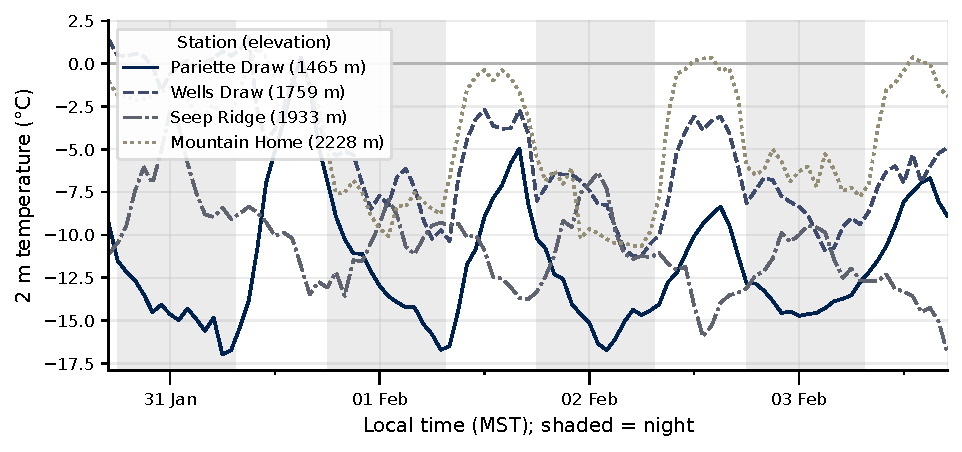
\includegraphics[width=\textwidth]{figures/obs_temp_timeseries_feb0102.pdf}
\caption{Observed 2 m-temperature evolution at four stations spanning the Uinta Basin floor and higher benches.
The shaded intervals indicate local night.
The sites provide elevation-spanning context but do not measure the full basin volume.}
\label{fig:observed-evolution}
\end{figure}

\subsection{Response to Driving Analysis across Feedback Modes}

The GFS-driven run produced a weaker horizontal bench-minus-floor potential-temperature contrast than the otherwise matched NAM-driven run throughout the evaluation window (Figure~\ref{fig:bulk-contrast}).
The observed contrast ranged from 12.63 to 20.21 K, the NAM run ranged from 16.44 to 18.07 K, and the GFS run ranged from 7.35 to 11.74 K.
These values describe a horizontal station contrast and are not interpreted as free-air inversion depths.

\begin{figure}[H]
\centering
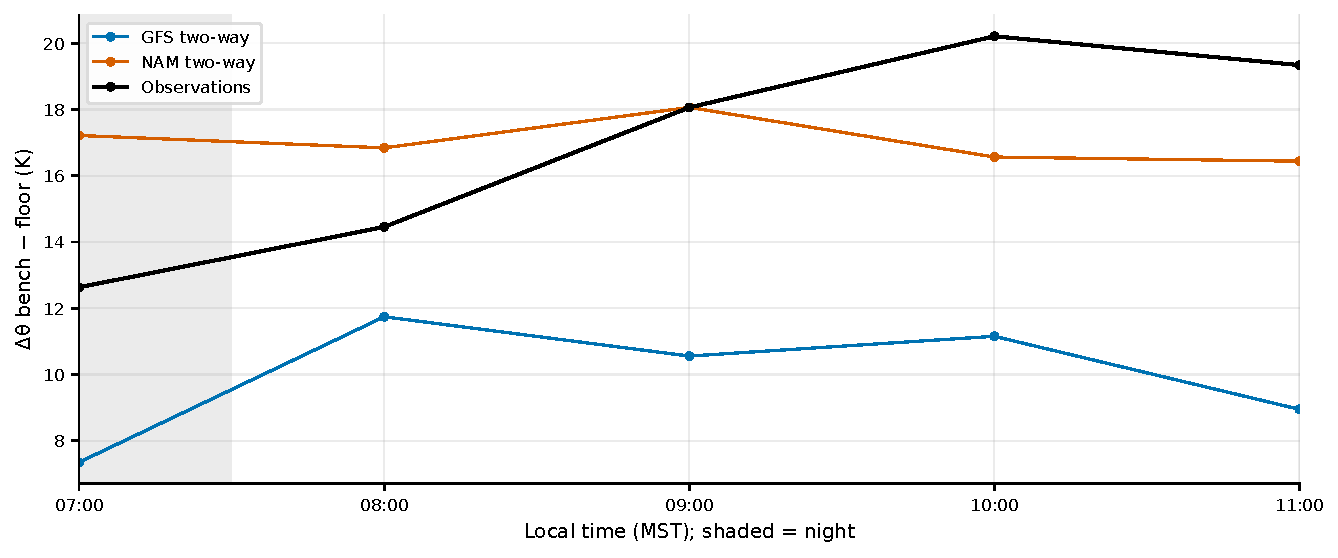
\includegraphics[width=\textwidth]{figures/wrf_inversion_index_feb0102_gfs2way_vs_nam2way_d02_14to18.pdf}
\caption{Observed and modeled Mountain Home-minus-Pariette Draw potential-temperature contrast during the matched evaluation window.
The 8 K line is a literature yardstick rather than a case-specific physical threshold.}
\label{fig:bulk-contrast}
\end{figure}

Under two-way feedback, the mean hourly station-median 2 m-temperature bias was +2.09 \(^{\circ}\mathrm{C}\) for GFS and +0.40 \(^{\circ}\mathrm{C}\) for NAM.
Under one-way feedback, the corresponding biases were +2.51 and +0.60 \(^{\circ}\mathrm{C}\).
The paired GFS-minus-NAM bias difference was +1.79 \(^{\circ}\mathrm{C}\) with two-way feedback and +1.76 \(^{\circ}\mathrm{C}\) with one-way feedback.
The corresponding absolute-temperature-error differences were +1.41 and +1.50 \(^{\circ}\mathrm{C}\), respectively.
The 10 m-wind-bias differences were similarly positive at +0.91 and +0.96 m s$^{-1}$, although the absolute-wind-error intervals spanned zero in both feedback modes.

The common-AGL profiles showed the same structural separation (Figure~\ref{fig:retention-ventilation}).
Across the five hourly spatial medians, GFS-minus-NAM 50--500 m stability was -3.63 K under two-way feedback and -3.65 K under one-way feedback.
The respective two-hour block sensitivity intervals were -4.94 to -2.22 K and -5.01 to -2.15 K, with the same sign in all five hours for both contrasts.
GFS-minus-NAM transport wind was +0.79 m s$^{-1}$ under two-way feedback and +0.99 m s$^{-1}$ under one-way feedback.
The respective intervals were +0.58 to +0.99 m s$^{-1}$ and +0.82 to +1.18 m s$^{-1}$, again with the same sign in all five hours.
The native PBL-height contrast changed sign and its interval spanned zero in both feedback modes, so PBLH alone did not explain the stability and transport-wind separation.

\begin{figure}[H]
\centering
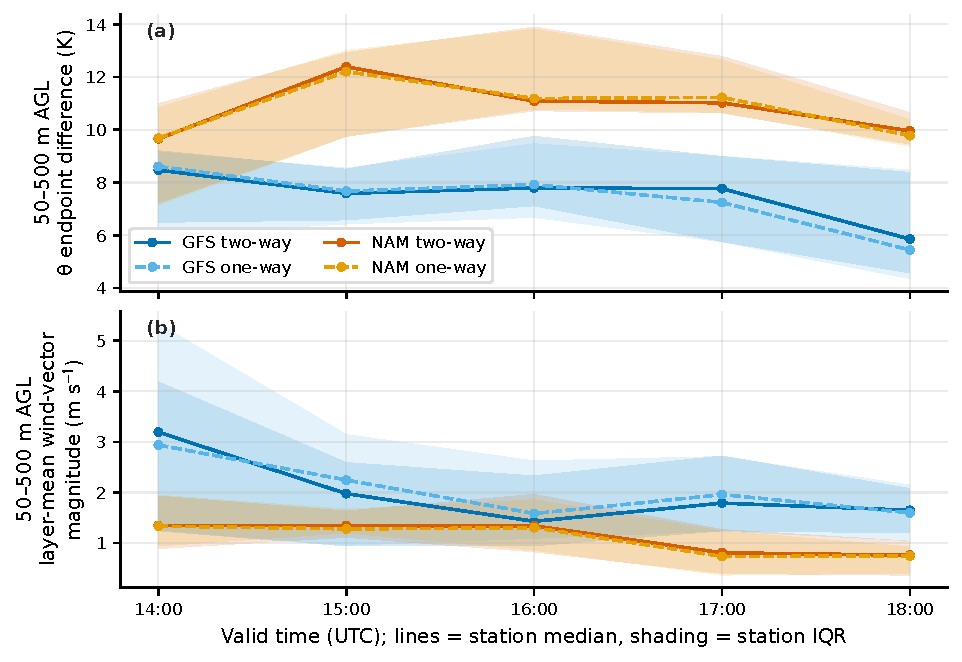
\includegraphics[width=\textwidth]{figures/wrf_retention_ventilation_d02_14to18.pdf}
\caption{Time evolution of station-column medians and interquartile ranges for 50--500 m AGL potential-temperature stability, fixed-layer transport wind, and native WRF PBL height.
Solid lines denote two-way feedback and dashed lines denote one-way feedback.
The GFS--NAM separation persists under both feedback modes, whereas the within-source feedback response is much smaller.}
\label{fig:retention-ventilation}
\end{figure}

\subsection{Response to Nest Feedback}

The within-source feedback responses were small relative to the driving-analysis response, but they were not identical between forcing families.
For NAM, one-way minus two-way was +0.002 K for 50--500 m stability and +0.006 m s$^{-1}$ for transport wind, with both block sensitivity intervals spanning zero.
For GFS, one-way minus two-way was -0.066 K for stability and +0.104 m s$^{-1}$ for transport wind, with respective intervals of -0.118 to -0.019 K and +0.051 to +0.152 m s$^{-1}$.
The paired forcing-by-feedback interaction was -0.103 K for stability and +0.097 m s$^{-1}$ for transport wind, with respective descriptive intervals of -0.176 to -0.031 K and +0.053 to +0.137 m s$^{-1}$.
The interaction in 2 m-temperature bias was only +0.041 \(^{\circ}\mathrm{C}\), and the PBL-height interaction interval spanned zero.
These results show a modest source-conditioned feedback response but bound it only for the present five-hour d02 sample; they do not establish general equivalence between one-way and two-way nesting.

\section{Discussion}

The driving analysis was the dominant tested control on the short-window cold-pool structure under both feedback modes.
The GFS-driven solutions combined larger warm surface errors, weaker 50--500 m stability, and stronger fixed-layer transport wind than their NAM-driven counterparts.
Those differences describe the meteorological state supplied to a downstream chemistry model, but the present experiment cannot partition the response between the 12:00 UTC initial state and the subsequent lateral boundary conditions.

Replicating the GFS--NAM separation under one-way and two-way feedback shows that the primary result is not an artifact of the selected feedback direction in this experiment.
The NAM feedback response was nearly null, while the GFS response and factorial interaction were coherent but small relative to the forcing contrast.
This does not show that feedback is unimportant for longer forecasts, the 333 m nest interior, different domain geometry, or other synoptic conditions.
The current resolution ladder, nudging lineage, terrain experiments, and PBL treatments were therefore excluded from the first-draft Results rather than used as additional nominal sensitivities.

For air-chemistry applications, the relevant implication is that the GFS-driven run supplied a less stable and more strongly ventilated lower layer during the evaluated window.
Such a state increases the atmospheric volume available for dilution and can hinder modeled near-surface accumulation, but it does not establish that meteorology is the only or dominant source of winter-ozone error.
Emissions, deposition, photolysis, snow representation, and chemical mechanisms remain material uncertainties.

The principal limitation is temporal scope.
Five post-spin-up hours can demonstrate a coherent structural difference but cannot establish cold-pool persistence across multiple diurnal cycles or the full ozone-accumulation period.
The station columns also sample fixed locations rather than basin volume, and the observed bench-minus-floor contrast is horizontal rather than a colocated sounding.

\section{Conclusions}

For the matched 2 February 2013 simulations, the driving analysis materially affected the short-window cold-pool state under both one-way and two-way nest feedback.
The GFS-driven simulations were warmer at the surface, less stable from 50 to 500 m AGL, and more strongly ventilated than the NAM-driven simulations.
Nest feedback produced a nearly null response under NAM forcing and a small source-conditioned response under GFS forcing, without approaching the magnitude of the driving-analysis contrast.
These findings provide a meteorological basis for later coupled modeling while remaining limited to a five-hour free-forecast comparison and leaving chemical and inventory uncertainties unresolved.

\vspace{6pt}

\institutionalreview{Not applicable.}
\informedconsent{Not applicable.}

\begin{adjustwidth}{-\extralength}{0cm}
\reftitle{References}
\bibliography{paperpile}
\PublishersNote{}
\end{adjustwidth}

\end{document}
